\documentclass[12pt,a4paper]{report}

%adjust your page margins here
\usepackage[top=15mm, bottom=22mm, left=30mm,right=20mm]{geometry} % setting the page alignment with this package
\usepackage[pdftex]{graphicx} %for embedding images
\usepackage[%dvips, % commented for pdflatex
bookmarks,  colorlinks=false]{hyperref} %for creating links in the pdf version and other additional pdf attributes, no effect on the printed document
\hypersetup{%
    pdfborder = {0 0 0}
}
\usepackage[final]{pdfpages} %for embedding another pdf, remove if not required
\usepackage{float} %used for figure placement with H as a parameter
\usepackage{hyperref}
\usepackage{pslatex} % for times new roman, old package, but works
\usepackage{array} % for making text bold in table
\usepackage{setspace}
\usepackage{float}
\usepackage{enumerate} % list numbering
\usepackage{longtable} % making tables that runs across pages
\usepackage{ragged2e}  % package for text justification
\usepackage{amsmath}  % package for maths 
\usepackage{makeidx} % package for making index  
\usepackage{showidx} % print index
\usepackage[font=small,labelfont=bf]{caption}
\usepackage[utf8]{inputenc}
\makeindex
\def\figurename{\textbf{Figure }}

\usepackage{listings}
\usepackage{color}

\usepackage{hhline}

\usepackage{graphicx}
\graphicspath{ {images/} }

\definecolor{dkgreen}{rgb}{0,0.6,0}
\definecolor{gray}{rgb}{0.5,0.5,0.5}
\definecolor{mauve}{rgb}{0.58,0,0.82}
 
\lstset{ %
  language=Java,                % the language of the code
  basicstyle=\footnotesize,           % the size of the fonts that are used for the code
  numbers=left,                   % where to put the line-numbers
  numberstyle=\tiny\color{gray},  % the style that is used for the line-numbers
  stepnumber=1,                   % each line is numbered
  numbersep=5pt,                  % how far the line-numbers are from the code
  backgroundcolor=\color{white},      % choose the background color. You must add \usepackage{color}
  showspaces=false,               % show spaces adding particular underscores
  showstringspaces=false,         % underline spaces within strings
  showtabs=false,                 % show tabs within strings adding particular underscores
  frame=single,                   % adds a frame around the code
  rulecolor=\color{black},        % if not set, the frame-color may be changed on line-breaks within not-black text (e.g. commens (green here))
  tabsize=2,                      % sets default tabsize to 2 spaces
  captionpos=b,                   % sets the caption-position to bottom
  breaklines=true,                % sets automatic line breaking
  breakatwhitespace=false,        % sets if automatic breaks should only happen at whitespace
  title=\lstname,                   % show the filename of files included with \lstinputlisting;
                                  % also try caption instead of title
  keywordstyle=\color{blue},          % keyword style
  commentstyle=\color{dkgreen},       % comment style
  stringstyle=\color{mauve},         % string literal style
  escapeinside={\%*}{*)},            % if you want to add a comment within your code
  morekeywords={*,...}               % if you want to add more keywords to the set
}

%For the header and footer
\usepackage{fancyhdr}
\fancypagestyle{plain}{%
\fancyfoot[L]{\emph{Department of Information Technology, DBIT, Mumbai}} % except the center
\fancyfoot[R]{\thepage}
\renewcommand{\headrulewidth}{0.4pt}
\renewcommand{\footrulewidth}{0.4pt}
}

\pagestyle{fancy}

%\rhead{\emph{NAME OF PROJECT}}

\fancyfoot[LO,LE]{\emph{Department of Information Technology, DBIT, Mumbai}}
\cfoot{}
\fancyfoot[RO, RE]{\thepage}
\renewcommand{\headrulewidth}{0.4pt}
\renewcommand{\footrulewidth}{0.4pt}
%For the header and footer Over

%Page Border
\usepackage{pgf}
\usepackage{pgfpages}

\pgfpagesdeclarelayout{boxed}
{
  \edef\pgfpageoptionborder{0pt}
}
{
  \pgfpagesphysicalpageoptions
  {%
    logical pages=1,%
  }
  \pgfpageslogicalpageoptions{1}
  {
    border code=\pgfsetlinewidth{2pt}\pgfstroke,%
    border shrink=\pgfpageoptionborder,%
    resized width=.95\pgfphysicalwidth,%
    resized height=.95\pgfphysicalheight,%
    center=\pgfpoint{.5\pgfphysicalwidth}{.5\pgfphysicalheight}%
  }%
}
\pgfpagesuselayout{boxed}
\setlength{\parindent}{1cm}
%GLOBAL SETTINGS OVER, DOCUMENT BEGINS
\begin{document}
\renewcommand\bibname{References}
\lhead{ }




%FROM HERE YOUR PAGES START GETTING ADDED

% includes the cover page
\newpage
\begin{center}
\thispagestyle{empty}
\LARGE{\textbf{SoftPlag}}\\[0.5cm]
\vspace{0.5cm}
\Large{\textbf{\\Submitted in partial fulfillment of the requirements}}
\vspace{0.5cm}
\Large{\textbf{\\of the degree of}}
\vspace{0.5cm}
\LARGE{\textbf{\\Bachelor of Engineering}}
\vspace{0.5cm}
\Large{\textbf{\\by}}
\vspace{0.5cm}
\Large{\textbf{\\Deven Bhalerao\\}}
\Large{\textbf{\\Roll No. 05 \\}}
\vspace{0.5cm}
\Large{\textbf{Supervisor:}}\\
\vspace{0.5cm}
\Large{\textbf{Prof. Prasad Padalkar}}\\
\vspace{1cm}
\includegraphics[scale=0.5]{project/images/jscoe_logo}\\
\vspace{1cm}
\Large{\textbf{Department of Information Technology}}\\
\vspace{0.5cm}
\Large{\textbf{Don Bosco Institute of Technology}}\\
%\large{\textbf{Vidyavihar Station Road, Mumbai - 400070}}
\large{\textbf{\\2016-2017}}\\
\vspace{1cm}
\Large{\textbf{AFFILIATED TO\\}}
\vspace{0.5cm}
\LARGE{\textbf{UNIVERSITY OF MUMBAI}}
\newpage
\end{center}
\newpage

%\input{project/title.tex}
%\newpage


% includes the certificate page
\begin{center}
\thispagestyle{empty}

\LARGE{\textbf{DON BOSCO INSTITUTE OF TECHNOLOGY}} \\ 
\large{\textbf{Vidyavihar Station Road, Mumbai - 400070}}\\[0.5cm]
\Large{\textbf{Department of Information Technology}}\\[1.5cm]

%\includegraphics[scale=0.5]{project/images/jscoe_logo}\\[0.5cm]

{\Huge \textbf{CERTIFICATE}}\\[0.5cm]
\end{center}
\linespread{1.13}

\large{\justify{This is to certify that the project entitled }\textbf{\Large{"SoftPlag"}} is a bonafide  work of  \\

\begin{table}[h]
\centering
\large{
\begin{tabular}{>{\bfseries}lc>{\bfseries}r}
Deven Bhalerao & & 05 \\Manish Jain & & 28 \\Vishal Jha & & 29\\Kunal Naik & & 45\\
\end{tabular}}
\end{table}

\justify submitted to the University of Mumbai in partial fulfillment of the requirement for the award of the degree of \textbf{\Large{Undergraduate}} in \textbf{\Large{Bachelor of Information Technology}} \\[0.25cm]
\large{\textbf{Date:\hspace*{1.0cm}/\hspace*{1.0cm}/}}\\
%\large{\textbf{Date:\date{}}}
\begin{spacing}{0}
\vspace{2.0cm}
\large{\textbf{Prof. Prasad Padalkar}}\hspace*{1.8in}\large{\textbf{}}\\
\hspace*{0.7in}\textbf{Supervisor}\hspace*{2.5in}\textbf{}\\[3cm]

\large{\textbf{Prof. Janhavi Baikerikar}}\hspace*{1.7in}\large{\textbf{Dr. Prasanna Nambiar}}\\
\hspace*{0.3in}\textbf{HOD, IT Department}\hspace*{2.5in}\textbf{Principal}\\[3cm]

%\hspace*{0.5cm}\large{\textbf{(Prof. HOD NAME)}}\hspace*{0.8in}\large{\textbf{(Dr. PRINCIPAL NAME)}}\\
%\textbf{HOD, Computer Department}\hspace*{0.8in}\textbf{Principal}\hspace*{1.1in}
\end{spacing} 
\newpage

% includes the Approval page
\begin{center}
\thispagestyle{empty}

\LARGE{\textbf{DON BOSCO INSTITUTE OF TECHNOLOGY}} \\ 
\large{\textbf{Vidyavihar Station Road, Mumbai - 400070}}\\[0.5cm]
\Large{\textbf{Department of Information Technology}}\\[1.5cm]

%\includegraphics[scale=0.5]{project/images/jscoe_logo}\\[0.5cm]

{\Huge \textbf{Project Report Approval for B.E.}}\\[0.5cm]
\end{center}
\linespread{1.13}

\large{\justify{This project report entitled }\textbf{\Large{"SoftPlag"}} by \textbf{\Large{Deven Bhalerao, Manish Jain, Vishal Jha, Kunal Naik}} is approved for the degree of \textbf{\Large{Bachelor of Engineering in Information Technology}}
%\vspace{0.25cm}
\begin{flushright}
\Large{\textbf{(Examiner's Name and Signature)}}\\[1cm]
\hspace*{0.7in}\textbf{1. ---------------------------------------}\\[1cm]
\hspace*{0.7in}\textbf{2. ---------------------------------------}\\[2cm]
\Large{\textbf{(Supervisor's Name and Signature)}}\\[1cm]
\hspace*{0.7in}\textbf{1. ---------------------------------------}\\[1cm]
\Large{\textbf{(Chairman)}}\\[1cm]
%\vspace{0.25cm}
\hspace*{0.7in}\textbf{1. ---------------------------------------}\\[1cm]
\end{flushright}
\justify\large{\textbf{Date:}}\\
\justify\large{\textbf{Place: }} 
\newpage

% includes the 

\begin{center}
\thispagestyle{empty}

\LARGE{\textbf{DON BOSCO INSTITUTE OF TECHNOLOGY}} \\ 
\large{\textbf{Vidyavihar Station Road, Mumbai - 400070}}\\[0.5cm]
\Large{\textbf{Department of Information Technology}}\\[1.5cm]

%\includegraphics[scale=0.5]{project/images/jscoe_logo}\\[0.5cm]

{\Huge \textbf{Declaration}}\\[0.5cm]
\end{center}
\linespread{1.13}

\large{\justify{I declare that this written submission represents my ideas in my own words and where others' ideas or words have been included, I have adequately cited and referenced the original sources. I also declare that I have adhered to all principles of academic honesty and integrity and have not misrepresented or fabricated or falsified any idea / data / fact / source in my submission. I understand that any violation of the above will be cause for disciplinary action by the Institute and can also evoke penal action from the sources which have thus not been properly cited or from whom proper permission has not been taken when needed. }

\begin{spacing}{0}
\vspace{3.0cm}
%\begin{justify}
\hspace*{3.6in}\Large{\textbf{(---------------------------- )}}\\
\vspace{1.0cm}
\hspace*{4.5in}\textbf{(Deven Bhalerao)}\\[1cm]

%\end{justify}
\end{spacing}
\justify\large{\textbf{Date:}}
 
\newpage

% includes the acknowledgements page
%\begin{center}
\thispagestyle{empty}
\LARGE{\textbf{Acknowledgements}}\\[1cm]
\end{center}
\linespread{1.13}
\large{\paragraph{}

This project was supported by Don Bosco Institute of Technology. We thank our teachers who provided insight and expertise that greatly assisted the project.\\
We thank Prof. Prasad Padalkar for assistance with forming the vision for our project.\\
We would also like to show our gratitude to the IT department teachers for sharing their pearls of wisdom with us during the course of this project. 




\begin{spacing}{0}
\vspace{3.0cm}
%\begin{justify}
\hspace*{3.6in}\Large{\textbf{(---------------------------- )}}\\
\vspace{1.0cm}
\hspace*{4.5in}\textbf{(Signature)}\\[1cm]
\hspace*{3.8in}\Large{\textbf{(---------------------------- )}}\\
\vspace{0.5cm}
\hspace*{3.8in}\textbf{(Deven Bhalerao[05])}\\[1cm]
%\end{justify}
\end{spacing}
\justify\large{\textbf{Date:}}

 
%\newpage

\begin{center}
\thispagestyle{empty}
\vspace{2cm}
\LARGE{\textbf{ABSTRACT}}\\[1.0cm]
\end{center}
\thispagestyle{empty}
\large{\paragraph{}The purpose of this project is to detect plagiarism of source code in the files given by user. This plagiarism detection software will be able to detect high level plagiarism which involves minor changes in logic, changes in flow of program etc. as well as low level plagiarism which involves changing variable names, adding comments etc.
}


\large{\paragraph{}Plagiarism is widespread practice in both the software industry and the educational institutes. Companies face a constant risk of getting their code stolen by competitors and incurring a huge economic loss. Students in colleges and schools also indulge in plagiarism in their programming assignments . Plagiarism can be done easily and this makes a plagiarism detection software an extremely useful tool.}\\
\textbf{Keywords: }Plagiarism, Java % adds the Research Methodology page
\newpage

%TABLE OF CONTENTS AND LIST OF FIGURES ARE AUTOMATICALLY ADDED BY FOLLOWING COMMANDS
%ADD FIGURE OF TABLES IF YOU NEED TO, CHECK DOCUMENTATION
\pagenumbering{roman} %numbering before main content starts


%To reset the Header & Footer for TOC and LOF
\pagestyle{empty}
\addtocontents{toc}{\protect\thispagestyle{empty}}
\tableofcontents % adds Index Page

\addtocontents{lof}{\protect\thispagestyle{empty}}
\listoffigures % adds List of Figures

\addtocontents{lot}{\protect\thispagestyle{empty}}
\listoftables % adds List of tables

%And reset back the settings we choose for Header and Footer
\pagestyle{fancy}

\newpage
\pagenumbering{arabic} %reset numbering to normal for the main content

\chapter{Introduction}
 \section{Problem Statement}

To develop a tool for detecting plagiarism in software source code using
the machine learning algorithms.
 \section{Scope of the Project}

 \begin{itemize}
\item For the first level of implementation , tool will be on a local machine for
checking plagiarism.
\item The source and target program should be in Java.
 \end{itemize}
 \section{Current Scenario}
\begin{table}[]
\centering
\begin{tabular}{|l|l|l|l|l|}
\hline
          & MOSS             & SHERLOCK                      & JPLAG                & CODEMATCH                     \\ \hline
Cost      & Free             & Open Source                   & Free                 & It is a Commercial Tool       \\ \hline
Safety    & Sign-in Required & Executes at Local machine     & Sign-in Required     & Executes at Local machine     \\ \hline
Service   & Internet         & Standalone                    & Web-Service          & Standalone                    \\ \hline
Algorithm & Winowing         & Token Matching                & Greedy String Tiling & String Matching               \\ \hline
Speed     & Fast             & More files requires more time & Fast                 & More files requires more time \\ \hline
\end{tabular}
\end{table}
 \section{Need for the Proposed System}
The Role of Plagiarism detection in Education, Role of Plagiarism Detection in Software,Industry especially copyright of software.
 \section{Summary of the Results / Task completed }
Study of different Research Papers,Thesis on Source Code Plagiarism.
Survey on different source code plagiarism tools.
Implementation upto Level 3 Plagiarism (Rule-based).
 % adds the introduction page
				\chapter{Review of Literature }
				\section{Summary of the investigation in the published papers}
				
				\begin{itemize}
				\item \textbf{Computer Algorithms for Plagiarism Detection}
				
				Described the various levels of plagiarism and the different metrics(approaches) like Halstead metric, ACCUSE metric, FORTRAN programs, etc. This paper also compared different algorithms based on the software metrics used. The different levels of plagiarism defined in this paper will form the foundation of our project and we’ll be looking to detect plagiarism based on these levels.
				
				
				
				\begin{figure}[h]	
				\centering			
					\includegraphics[width=0.8\textwidth]{LevelDiag}
	  				\label{fig:Level1}
	  				\caption{Spectrum of Plagiarism}
					\end{figure}
				
				
				\pagebreak
				
				\item \textbf{A Comparison of Similarity Techniques for Detecting Source Code Plagiarism}
				
				This paper outlines different modern approaches to software similarity measurement. Algorithms like Levenshtein edit distance, Tree edit distance and graph edit distance were discussed. Knowledge of different approaches was gained and this will help us choose our approach.
				
				\item  \textbf{An Approach to Source-Code Plagiarism Detection and Investigation Using Latent Semantic Analysis}
				
				Latent Semantic Analysis, a statistical approach to detecting similarity is analysed in-depth in this paper. This paper also has an exhaustive description of what constitutes Plagiarism which includes surveys and research papers. Deeper understanding of Plagiarism was made possible by this research paper.
				
				\item  \textbf{Plagiarism Detection in Java Code}
				
				This thesis gives a step-by-step procedure on how to detect plagiarism in java source code using the Levenshtein Edit distance algorithm. It uses different normalization techniques and demonstrates these techniques using examples. Normalization techniques shown inn this thesis will be used in our project.
				
				\item \textbf{Source Code Plagiarism Detection ‘SCPDet’: A Review}
				
				In this paper author describes the real meaning of source code plagiarism and  then described the different source code plagiarism detection tools and compared its function, characteristics and technique. In the last phase, authors discussed the different research papers and compared in tabular form with its technique, method, characteristics, functionality and its result.
				
				\end{itemize} 
				
\newpage
				\section{Comparison between the tools / methods / algorithms}\begin{table}[!htbp]
				  \centering
				  \caption{Compression of four source code detection tools with its characteristics, function and technique}
				  \label{tab:table1}
				  \begin{tabular}{|p{3cm}|p{3cm}|p{3cm}|p{3cm}|p{3cm}|}
				\hline 
				Tools & JPlag & SIM & MOSS & Plaggie \\ \hline
				
				Open Source Tools/Paid & NO & YES & NO & YES \\ \hline
				Local/online tool & Web & Local & Web & Local  \\ \hline
				Code Submit/File & Submit Code & Submit File & Submit
				Code & Submit Code  \\ \hline
				Lang. Support & 6 & 5 & 23 & 1 \\ \hline
				Expandability & No & Yes & No & No \\ \hline
				Founded in Year & 1996 & 1989 & 1994 & 2002 \\ \hline
				Founded By  & Guido Malpohl & Dick Grune & Aiken & Ahtiaine \\ \hline
				
				Technique & Greedy String Tiling and Optimization and Tokenization & Flax lexical analyzer & Winnowing technique & Greedy String Tiling and Tokenization \\ \hline	\end{tabular}
				
				\vspace{40 mm}
				
				  \centering
				  \caption{Comparison between different metrics : Structural Metrics and Similarity Metrics}
				  \label{tab:table2}
				  \begin{tabular}{|p{6cm}|p{6cm}|}
				\hline 
				Structural metrics & Similarity metrics  \\ \hline
				
				Structural metrics – no. of variables, no. of keywords, no. of loops, no. of comment lines & Similarity metrics – no. of characters per line, no of code lines, no. of blank lines \\ \hline
				
				Structural metrics represent information about programming constructs and elements used in the code. & Similarity metrics are indicative of the style used in programming and are effective in detecting plagiarism. \\ \hline	
				
				
				Lots of rudimentary plagiarism detection algorithms like Halstead use only structural metrics and are ineffective for larger programs. &  Modern approaches include algorithms that use a combination of structural and similarity metrics to detect plagiarism and are highly effective. \\ \hline 
				
				\end{tabular}
						
				
				
				\end{table}  
				
				
				
				
	\pagebreak
				
				\section{Algorithms}
				
				\begin{itemize}
				
				\item \textbf{Level 0 Plagiarism Pseudo-Code}
					\begin{figure}[h]
					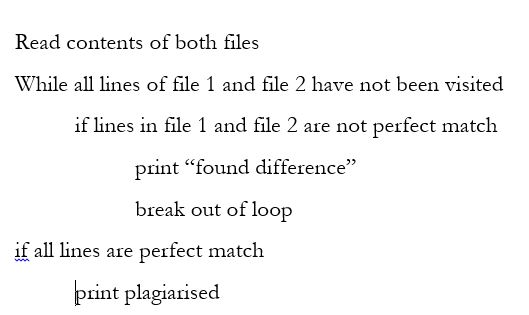
\includegraphics[width=0.8\textwidth]{Level0Alg}
	  				\label{fig:Level0}
	  				\end{figure}
	  				
				
				\item \textbf{Level 1 Plagisrism Pseudo-Code}
					\begin{figure}[!h]				
					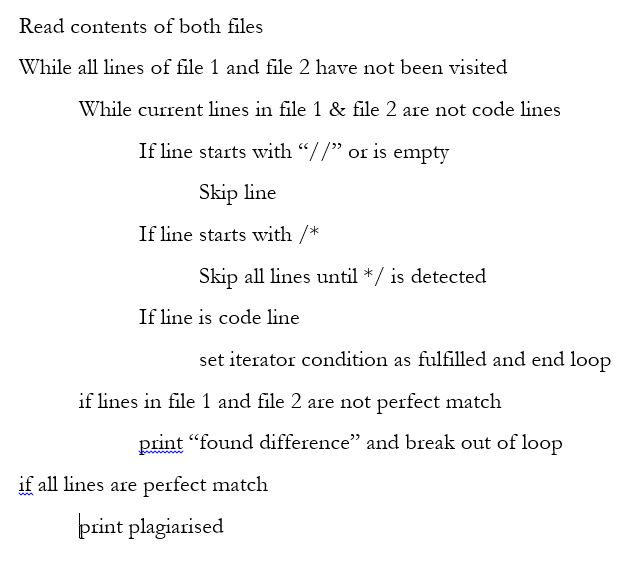
\includegraphics[width=0.8\textwidth]{Level1Alg}
	  				\label{fig:Level1}
					\end{figure}
					
				\pagebreak				
	
				\item \textbf{Level 3 Plagisrism Pseudo-Code}\\
					\begin{figure}[h]				
					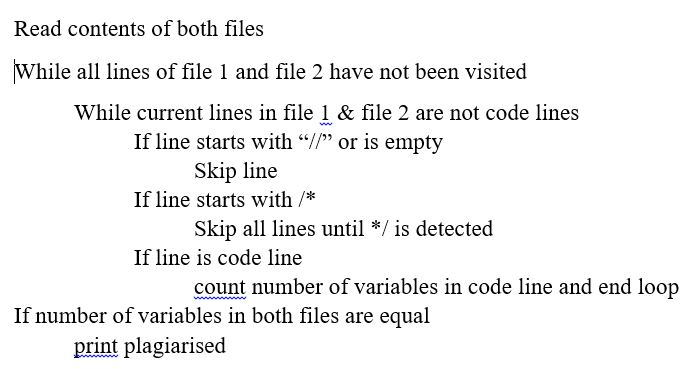
\includegraphics[width=0.8\textwidth]{Level3Alg}
	  				\label{fig:Level3}	
	  				\end{figure}		
				
				\end{itemize} 
				
				
				
				
				
				
				
				
				
				
				
				
				
				
				
				
				
				
				 % adds the Literature Survey page
\chapter{Analysis and Design}
\section{Methodology / Procedure adopted}
\begin{itemize}
\item The common ways adopted by people for plagiarizing the code are:
\begin{enumerate}
 \item The original source code can be replicated as it is.
 \item Addition of comments in the source code.
 \item Modification in identifiers. 
 \item Chane in variable position.
 \item The procedure combination can be done in source code.
 \item Program statements can be changed by some modifications.
 \item Control Logic can be modified.
 \end{enumerate}
\item Describe on the development methodology / model you would use. (E.g. Agile method or Iterative Model)
\begin{enumerate}
\item In Iterative model, iterative process starts with a simple implementation of a small set of the software requirements and iteratively enhances the evolving versions until the complete system is implemented and ready to be deployed.
\item An iterative life cycle model does not attempt to start with a full specification of requirements. Instead, development begins by specifying and implementing just part of the software, which is then reviewed in order to identify further requirements. This process is then repeated, producing a new version of the software at the end of each iteration of the model.\\
\end{enumerate}
\item How you intend manage the weekly meetings ? \\
The weekly meetings need to managed properly because in order to accomplish the goals desired, you will need to have a good strategic and tactical plan. In the meeting, plans may be decided by each team member and the procedure is been planned.
\item How do you intend to monitor and measure the progress of the project? \\ 
The monitoring and measure of progress of report is been done on basis of different modules. A schedule is maintained for each module to be complemented. Github is used for project monitoring ,as all the team members upload their work on completion. 
\end{itemize}
\section{Analysis}

Based on the requirements gathered, how was the feasibility study of the project carried out? \\
The project is about the detection of software source code plagiarism ,so the study carried out on the comparison of the different plagiarism software's which are based on rule based algorithms.\\
On comparison of different features of some software's.\\
The papers were referred for plagiarism detection, which gives the idea of different levels of plagiarism and defining the metrics for the programs.  \\
If any requirements, were modified why they were modified? \\

\subsection{Software / System Requirement Specification - IEEE format}
\textbf{Table of Contents}\\
\textbf{Revision History}\\
\textbf{1.\hspace{0.3cm}	Introduction}\\
\textbf{1.1\hspace{0.3cm} Purpose}\\
\textbf{1.2 \hspace{0.3cm} Document Conventions}\\
\textbf{1.3 \hspace{0.3cm} Intended Audience and Reading Suggestions}\\
\textbf{1.4 \hspace{0.3cm} Product Scope}\\
\textbf{1.5 \hspace{0.3cm} References}\\
\textbf{2.\hspace{0.3cm}	Overall Description}\\
\textbf{2.1	\hspace{0.3cm}Product Perspective}\\
\textbf{2.2\hspace{0.3cm}	Product Functions}\\
\textbf{2.3	\hspace{0.3cm}User Classes and Characteristics}\\
\textbf{2.4	\hspace{0.3cm}Operating Environment}\\
\textbf{2.5\hspace{0.3cm}	Design and Implementation Constraints}\\
\textbf{3.	\hspace{0.3cm}External Interface Requirements}\\
\textbf{3.1	\hspace{0.3cm}User Interfaces}\\
\textbf{3.2	\hspace{0.3cm}Hardware Interfaces}\\
\textbf{3.3	\hspace{0.3cm}Software Interfaces}\\
\textbf{4.\hspace{0.3cm}	System Features}\\
\textbf{4.1	\hspace{0.3cm}System Feature 1}\\
\textbf{5.\hspace{0.3cm}	Other Nonfunctional Requirements}\\
\textbf{5.1	\hspace{0.3cm}Software Quality Attributes}\\
\textbf{5.2	\hspace{0.3cm}Business Rules}\\
\textbf{Appendix A: Glossary}\\
\textbf{Appendix B: Analysis Models}\\
\textbf{Appendix C: To Be Determined List}\\\\

\textbf{\huge Revision History}\\

\begin{center}
\begin{tabular}{ |c|c|c|c| } 

 \hline
 Name & Date & Reason For Changes & Version \\ [0.5ex] 
  \hline
  &  &  &  \\ 
  \hline
  &  &   & \\ 
  \hline
\end{tabular}
\end{center}
\textbf{1.	Introduction}\\
 Plagiarism Detection is the process of finding  instances of plagiarism within a work or document. The worldwide and widespread use of computers and  Internet has made it easier to plagiarize the work of others. Most cases of plagiarism are found in academia, where source code, art designs, documents like essays , reports etc. So Our Software is use to find plagiarism in source code.\\
In our plagiarism detection software detection of plagiarism is software-assisted. Software-assisted detection allows vast collections of documents to be compared to each other, making successful detection much more likely. Software assisted reduces effort and time required for plagiarism detection. \\
\textbf{1.1	Purpose }\\
Plagiarism means  the practice of taking someone else's work or ideas and passing them off as one's own. Plagiarism detection tool is useful to detect plagiarism. Plagiarism are found in colleges, organization or any institute level. So our software is useful for colleges ,Organizations, Institutes to find plagiarism in their respective work area. Our software tool  only use to find plagiarism in source code. Our Aim to reduce plagiarism in all field. so everyone will look to think and present their idea or work instead of showing others ideas or work.\\
\textbf{1.2	Document Conventions}\\
// <Describe any standards or typographical conventions that were followed when writing this SRS, such as fonts or highlighting that have special significance. For example, state whether priorities  for higher-level requirements are assumed to be inherited by detailed requirements, or whether every requirement statement is to have its own priority.>\\
\textbf{1.3	Intended Audience and Reading Suggestions}\\
This Document is intended for developers ,designers ,tester ,project managers, users and documentation writers. Document contains scope of product ,product Perspective ,functions, hardware and software specification ,features of product.\\
\textbf{1.4	Product Scope}\\
Plagiarism detection software take user input as an java file and it checks  with  repository present on local machine and display result. Scope  of product is only java file can be check to decide it  is plagiarized or not. The source  and target program should be in Java.\\
\textbf{1.5	References}\\
// 
<List any other documents or Web addresses to which this SRS refers. These may include user interface style guides, contracts, standards, system requirements specifications, use case documents, or a vision and scope document. Provide enough information so that the reader could access a copy of each reference, including title, author, version number, date, and source or location.>\\\\
\textbf{2.	Overall Description}\\
\textbf{2.1	Product Perspective}\\
Plagiarism detection software is used to check plagiarism in source code in java language only. It is new ,self-contained product. It will able to detect all levels of plagiarism in java programming language. It will implement and extends all features that are not present in other tool and required for plagiarism detection. What Metrics we are  consider to check whether file is plagiarized or not those all metrics are important parameter of our product.  It will help to reduce plagiarism in an institutes, colleges and organizations.\\
\textbf{2.2	Product Functions}\\
In Plagiarism detection software from user system will take java program file to check whether it is plagiarized or not. System will compare it with program in repository and if it is match then it will show that file it plagiarized and if it does not match then system shows file is not plagiarized. Main function of it that it will detect all levels of plagiarism. Effective for detecting plagiarized file. \\
\textbf{2.3	User Classes and Characteristics}\\
//
<Identify the various user classes that you anticipate will use this product. User classes may be differentiated based on frequency of use, subset of product functions used, technical expertise, security or privilege levels, educational level, or experience. Describe the pertinent characteristics of each user class. Certain requirements may pertain only to certain user classes. Distinguish the most important user classes for this product from those who are less important to satisfy.>\\
\textbf{2.4	Operating Environment}\\
Software Requirement :\\
Java Runtime Environment\\
Operating environment –Windows /Linux\\\\
Hardware Requirement:\\
Minimum memory – 512 Mb  RAM\\
Hard disk space-1 GB\\
\textbf{2.5	Design and Implementation Constraints}\\
Project  Scope is only for java language so to work this tool properly both user file and files which are present in repositories should be  in java .\\\\
\textbf{3.	External Interface Requirements}\\
\textbf{3.1	User Interfaces}\\
There will be an screen where user has to upload file for plagiarism detection. So will give an upload button to user to upload any java file an then will compare it with our repository  and then display result about it. Result will be shown in an percentage format based on levels of plagiarism.\\
\textbf{3.2	Hardware Interfaces}\\
For this software minimum 512 Mb RAM and 1 GB hard disk is required. It can be use in windows or linux operating systems.\\
\textbf{3.3	Software Interfaces}\\
Plagiarism detection software contain repositories which has no of java files. So whenever user gives an input it will compare it with repository files and display result.\\\\
\textbf{4.	System Features}\\
\textbf{4.1	Level wise Plagiarism Detection }\\
\textbf{4.1.1	Description and Priority}\\
In our system it will detect plagiarism in user file level by level by  checking all  plagiarism levels conditions.\\
Level wise plagiarism detection feature has high priority in our project. \\
\textbf{4.1.2  Stimulus/Response Sequences}\\
Here input from user will take like any java file then system will process it. compare With it repository including all levels of plagiarism. Then result will be display to the user.\\
\textbf{4.1.3	Functional Requirements}\\
To work all functions of the system properly on user system. Java runtime environment should be installed on user machine to run software and to use all functionality . \\\\
\textbf{5.	Other Nonfunctional Requirements}\\
\textbf{5.1	Software Quality Attributes}\\
\textbf{Correctness:} When user give an input of an java file to check whether the file is plagiarized or not then system will shows an correct result to user by comparing it with an repository files.\\
\textbf{Reliability:} This will be an simple application even work in an minimum ram and space so it will not crash .\\
\textbf{Performance :}The performance of the system will be optimal. It will be easy to operate for an users.\\
\textbf{Usability:} We will make an software as simple as possible for the users understanding .So it is easy to use an software to any user.\\
\textbf{5.2	Business Rules}\\
//
<List any operating principles about the product, such as which individuals or roles can perform which functions under specific circumstances. These are not functional requirements in themselves, but they may imply certain functional requirements to enforce the rules.>\\\\




\section{Proposed System}

Give the details of your proposed system and architecture 
Advantage of the proposed system over the existing system

\subsection{Hardware / Software requirements}
Development Hardware / Software requirements \\\\
Software Requirements : \\
Java  JDK 1.4 or more \\
Operating System : Window/Linux\\
Front-End : Java Fx\\
Back-End : MySQL\\\\
Hardware Requirements :\\
Minimum Memory : 512 Mb RAM \\
Hard disk space : 1 GB\\\\
Deployment Hardware / Software requirements \\\\
Software Requirements : \\
Java Runtime Environment\\
Operating System : Window/Linux. \\\\
Hardware Requirements : \\
Minimum Memory : 512 Mb RAM \\
Hard disk space : 1 GB\\

\subsection{Design Details}

Different UML diagrams as per the project requirement (For e.g. Use Case Diagram)

\subsection{Implementation Plan}

Timeline chart is for Next semester 





\section{Proposed System}

Give the details of your proposed system and architecture 
Advantage of the proposed system over the existing system

\subsection{Hardware / Software requirements}
Development Hardware / Software requirements \\
Deployment Hardware / Software requirements \\

\subsection{Design Details}

Different UML diagrams as per the project requirement (For e.g. Use Case Diagram)

\subsection{Implementation Plan}

Timeline chart is for Next semester

\chapter{Results and Discussion }

\section{Result of Comparison for various levels for Execution time}
\begin{itemize}
\item Level One Plagiarism Detection.

  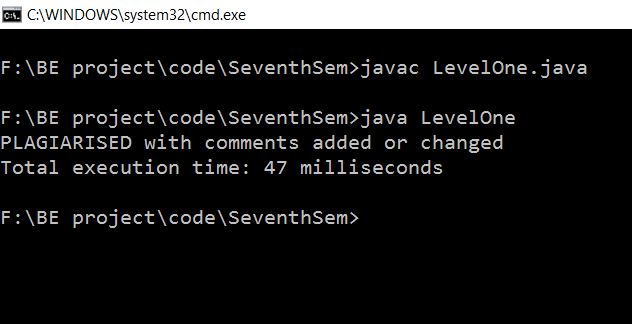
\includegraphics[width=.8\textwidth]{Level1}
  \label{fig:Level1}

\item Level Three Plagiarism Detection.

  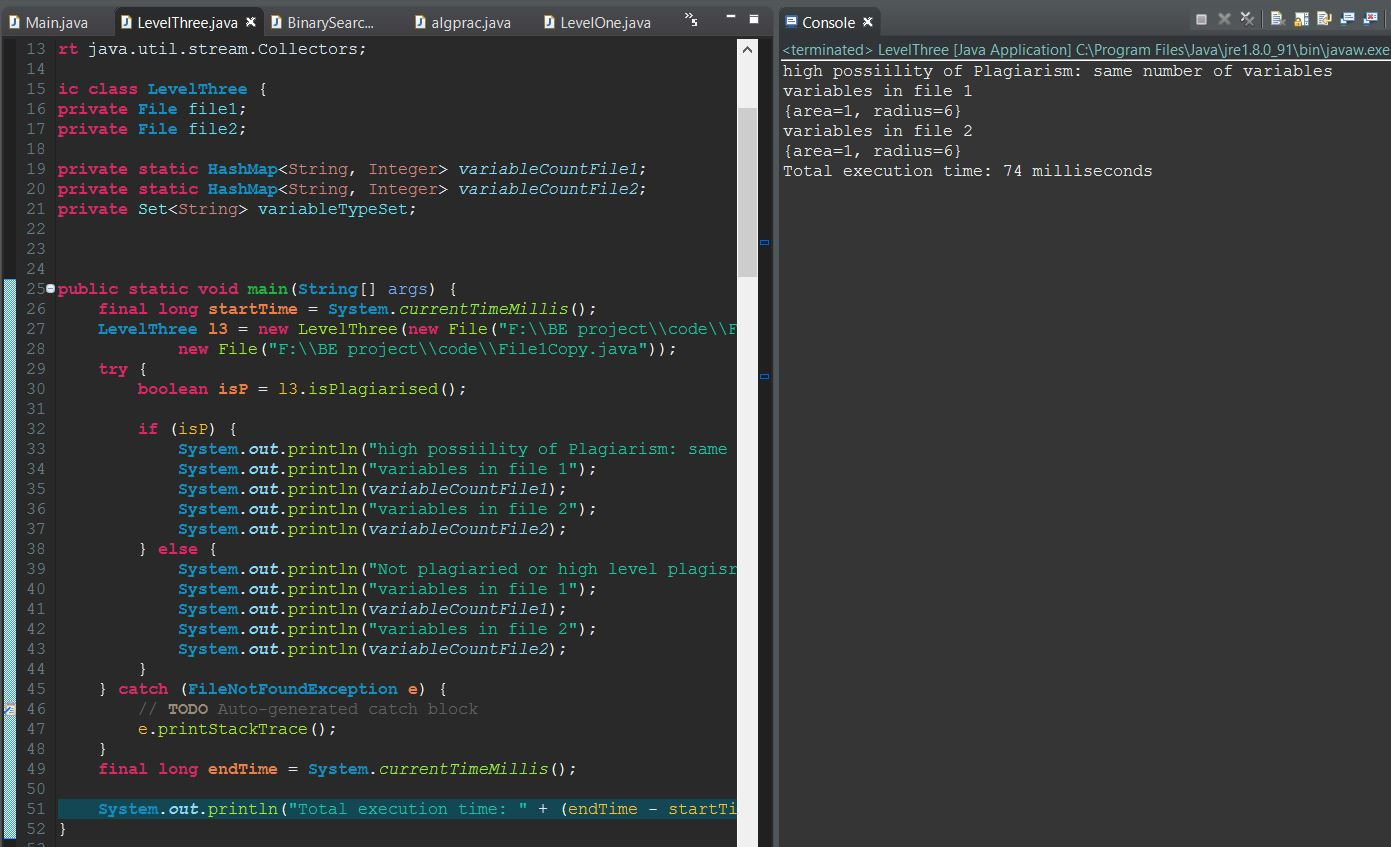
\includegraphics[width=.8\textwidth]{Level3}
  \label{fig:Level3}
  
\item Result from JPlag.



  \includegraphics[width=.8\textwidth]{JPlag}
  \label{fig:JPlag}
  
  
  
\item Result from MOSS.



  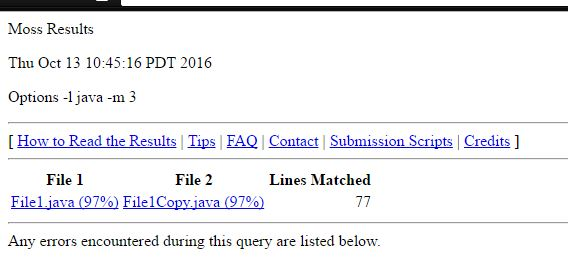
\includegraphics[width=.8\textwidth]{MOSS}
  \label{fig:MOSS}


\end{itemize}

\chapter{Conclusion}

SoftPlag is a useful tool to help detect plagiarism in source code.It is able to identify a wide range of plagiarism types which includes comment addition, changing names of variables and changing control flow of program.It can be used by both educational institutes as well as software companies to prevent plagiarism.


\newpage
	\begin{center}
	\thispagestyle{empty}
	\vspace{2cm}
	\LARGE{\textbf{Appendix - I}}\\[1.0cm]
	\end{center}
	
	\textbf{Software / System Requirement Specification - IEEE format}\\
	\textbf{Table of Contents}\\
	1.\hspace{0.3cm}	Introduction\\
	1.1\hspace{0.3cm} Purpose\\
	1.2 \hspace{0.3cm} Document Conventions\\
	1.3 \hspace{0.3cm} Intended Audience and Reading Suggestions\\
	1.4 \hspace{0.3cm} Product Scope\\
	1.5 \hspace{0.3cm} References\\
	2.\hspace{0.3cm}	Overall Description\\
	2.1	\hspace{0.3cm}Product Perspective\\
	2.2\hspace{0.3cm}	Product Functions\\
	2.3	\hspace{0.3cm}User Classes and Characteristics\\
	2.4	\hspace{0.3cm}Operating Environment\\
	2.5\hspace{0.3cm}	Design and Implementation Constraints\\
	3.	\hspace{0.3cm}External Interface Requirements\\
	3.1	\hspace{0.3cm}User Interfaces\\
	3.2	\hspace{0.3cm}Hardware Interfaces\\
	3.3	\hspace{0.3cm}Software Interfaces\\
	4.\hspace{0.3cm}	System Features\\
	4.1	\hspace{0.3cm}System Feature 1\\
	5.\hspace{0.3cm}	Other Nonfunctional Requirements\\
	5.1	\hspace{0.3cm}Software Quality Attributes\\
	5.2	\hspace{0.3cm}Business Rules\\
	
	\textbf{1.	Introduction}\\
	 Plagiarism Detection is the process of finding  instances of plagiarism within a work or document. The worldwide and widespread use of computers and  Internet has made it easier to plagiarize the work of others. Most cases of plagiarism are found in academia, where source code, art designs, documents like essays , reports etc. So Our Software is use to find plagiarism in source code.\\
	In our plagiarism detection software detection of plagiarism is software-assisted. Software-assisted detection allows vast collections of documents to be compared to each other, making successful detection much more likely. Software assisted reduces effort and time required for plagiarism detection. \\
	\textbf{1.1	Purpose }\\
	Plagiarism means  the practice of taking someone else's work or ideas and passing them off as one's own. Plagiarism detection tool is useful to detect plagiarism. Plagiarism are found in colleges, organization or any institute level. So our software is useful for colleges ,Organizations, Institutes to find plagiarism in their respective work area. Our software tool  only use to find plagiarism in source code. Our Aim to reduce plagiarism in all field. so everyone will look to think and present their idea or work instead of showing others ideas or work.\\
	
	\textbf{1.3	Intended Audience and Reading Suggestions}\\
	This Document is intended for developers ,designers ,tester ,project managers, users and documentation writers. Document contains scope of product ,product Perspective ,functions, hardware and software specification ,features of product.\\
	\textbf{1.4	Product Scope}\\
	Plagiarism detection software take user input as an java file and it checks  with  repository present on local machine and display result. Scope  of product is only java file can be check to decide it  is plagiarized or not. The source  and target program should be in Java.\\
	\textbf{1.5	References}\\
	 
	 
	 \begin{itemize}
	 
	\item Fonte, V. Martins, R. Henriques and D. da Cruz, 1st ed. Portugal, 1998, pp. 147-148.\\
	
	
	\item Cosma, Georgina. A Thesis Submitted In Partial Fulfilment Of The Requirements For The Degree Of Doctor Of Philosophy In Computer Science. 1st ed. Warwick: N.p., 2008. Print.\\
	
	\item Parker, Alan and James Hamblen. Computer Algorithms For Plagiarism Detection. 2nd ed. Atlanta: N.p., 1989. Print.\\
	\item Ali, Asim M. El Tahir and Vaclav Snase. Overview And Comparison Of Plagiarism Detection Tools. 1st ed. Czech Republic: N.p. Web.\\
	\item MUFTAH, AHMED JABR AHMED. Document Plagiarism Detection algorithm using semantic network. 1st ed. Malaysia: N.p., 2009. Print.\\
	\item Haider, Khurram Zeeshan, Tabassam Nawaz, and Ali Javed. Efficient Source Code Plagiarism Identification Based On Greedy String Tilling. 10th ed. Taxila: N.p., 2010. Web. 23 Aug. 2016.\\
	
	\end{itemize}
	\textbf{2.	Overall Description}\\
	\textbf{2.1	Product Perspective}\\
	Plagiarism detection software is used to check plagiarism in source code in java language only. It is new ,self-contained product. It will able to detect all levels of plagiarism in java programming language. It will implement and extends all features that are not present in other tool and required for plagiarism detection. What Metrics we are  consider to check whether file is plagiarized or not those all metrics are important parameter of our product.  It will help to reduce plagiarism in an institutes, colleges and organizations.\\
	\textbf{2.2	Product Functions}\\
	In Plagiarism detection software from user system will take java program file to check whether it is plagiarized or not. System will compare it with program in repository and if it is match then it will show that file it plagiarized and if it does not match then system shows file is not plagiarized. Main function of it that it will detect all levels of plagiarism. Effective for detecting plagiarized file. \\
	\textbf{2.4	Operating Environment}\\
	Software Requirement :\\
	Java Runtime Environment\\
	Operating environment –Windows /Linux\\
	Hardware Requirement:\\
	Minimum memory – 512 Mb  RAM\\
	Hard disk space-1 GB\\
	\textbf{2.5	Design and Implementation Constraints}\\
	Project  Scope is only for java language so to work this tool properly both user file and files which are present in repositories should be  in java .\\
	\textbf{3.	External Interface Requirements}\\
	\textbf{3.1	User Interfaces}\\
	There will be an screen where user has to upload file for plagiarism detection. So will give an upload button to user to upload any java file an then will compare it with our repository  and then display result about it. Result will be shown in an percentage format based on levels of plagiarism.\\
	\textbf{3.2	Hardware Interfaces}\\
	For this software minimum 512 Mb RAM and 1 GB hard disk is required. It can be use in windows or linux operating systems.\\
	\textbf{3.3	Software Interfaces}\\
	Plagiarism detection software contain repositories which has no of java files. So whenever user gives an input it will compare it with repository files and display result.\\
	\textbf{4.	System Features}\\
	\textbf{4.1	Level wise Plagiarism Detection }\\
	\textbf{4.1.1	Description and Priority}\\
	In our system it will detect plagiarism in user file level by level by  checking all  plagiarism levels conditions.\\
	Level wise plagiarism detection feature has high priority in our project. \\
	\textbf{4.1.2  Stimulus/Response Sequences}\\
	Here input from user will take like any java file then system will process it. compare With it repository including all levels of plagiarism. Then result will be display to the user.\\
	\textbf{4.1.3	Functional Requirements}\\
	To work all functions of the system properly on user system. Java runtime environment should be installed on user machine to run software and to use all functionality . \\
	\textbf{5.	Other Nonfunctional Requirements}\\
	\textbf{5.1	Software Quality Attributes}\\
	\textbf{Correctness:} When user give an input of an java file to check whether the file is plagiarized or not then system will shows an correct result to user by comparing it with an repository files.\\
	\textbf{Reliability:} This will be an simple application even work in an minimum ram and space so it will not crash .\\
	\textbf{Performance :}The performance of the system will be optimal. It will be easy to operate for an users.\\
	\textbf{Usability:} We will make an software as simple as possible for the users understanding .So it is easy to use an software to any user.\\

\newpage
\begin{thebibliography}{99}
\bibitem{ZHI06} Zhi Zhou, Member, IEEE, Gonzalo R. Arce, Fellow, IEEE, and Giovanni Di Crescenzo; \emph{Halftone Visual Cryptography}; IEEE TRANSACTIONS ON IMAGE PROCESSING, VOL. 15, NO. 8, AUGUST 2006

\bibitem{ZHI06}[D. Fonte, V. Martins, R. Henriques and D. da Cruz, 1st ed. Portugal, 1998, pp. 147-148.
\bibitem{ZHI06}Cosma, Georgina. A Thesis Submitted In Partial Fulfilment Of The Requirements For The Degree Of Doctor Of Philosophy In Computer Science. 1st ed. Warwick: N.p., 2008. Print.
\bibitem{ZHI06}Parker, Alan and James Hamblen. Computer Algorithms For Plagiarism Detection. 2nd ed. Atlanta: N.p., 1989. Print.
\bibitem{ZHI06}Ali, Asim M. El Tahir and Vaclav Snase. Overview And Comparison Of Plagiarism Detection Tools. 1st ed. Czech Republic: N.p. Web.
\bibitem{ZHI06}MUFTAH, AHMED JABR AHMED. Document Plagiarism Detection algorithm using semantic network. 1st ed. Malaysia: N.p., 2009. Print.
\bibitem{ZHI06}Haider, Khurram Zeeshan, Tabassam Nawaz, and Ali Javed. Efficient Source Code Plagiarism Identification Based On Greedy String Tilling. 10th ed. Taxila: N.p., 2010. Web. 23 Aug. 2016.

\end{thebibliography} % adds the References page
\newpage
\begin{center}
\thispagestyle{empty}
\LARGE{\textbf{Acknowledgements}}\\[1cm]
\end{center}
\linespread{1.13}
\large{\paragraph{}

This project was supported by Don Bosco Institute of Technology. We thank our teachers who provided insight and expertise that greatly assisted the project.\\
We thank Prof. Prasad Padalkar for assistance with forming the vision for our project.\\
We would also like to show our gratitude to the IT department teachers for sharing their pearls of wisdom with us during the course of this project. 




\begin{spacing}{0}
\vspace{3.0cm}
%\begin{justify}
\hspace*{3.6in}\Large{\textbf{(---------------------------- )}}\\
\vspace{1.0cm}
\hspace*{4.5in}\textbf{(Signature)}\\[1cm]
\hspace*{3.8in}\Large{\textbf{(---------------------------- )}}\\
\vspace{0.5cm}
\hspace*{3.8in}\textbf{(Deven Bhalerao[05])}\\[1cm]
%\end{justify}
\end{spacing}
\justify\large{\textbf{Date:}}

 
\printindex
\end{document}
